% Pagina originale 36
\pagina{36}
Affinché $y_\ell$ sia asintoticamente stabile:
\[
m_i(t)e^{p_it}\to0\quad\forall i,
\qquad e^{p_it}\to0\quad\Longrightarrow\quad\operatorname{Re}(p_i)<0\quad\forall i.
\]
\subsection*{Classificazione della stabilità di un sistema LTI in base ai poli di $G(s)$}
\begin{enumerate}
\item Sistema asintoticamente stabile $\Longleftrightarrow\forall i:\operatorname{Re}(p_i)<0$.
\item Sistema instabile $\Longleftrightarrow\exists p\in\{p_i\}:\operatorname{Re}(p)>0$, oppure
$\exists i:\operatorname{Re}(p_i)=0\land r_i\geq1$.
\item Sistema semplicemente stabile $\Longleftrightarrow\forall i:\operatorname{Re}(p_i)<0$, oppure
$(\operatorname{Re}(p_i)=0\land r_i=1)$.
\end{enumerate}
% La scansione scrive r_i >= 1 nel criterio di instabilità e r_i=1 nel criterio di stabilità semplice; disuguaglianza conservata.
\paragraph{Esempi}
\begin{center}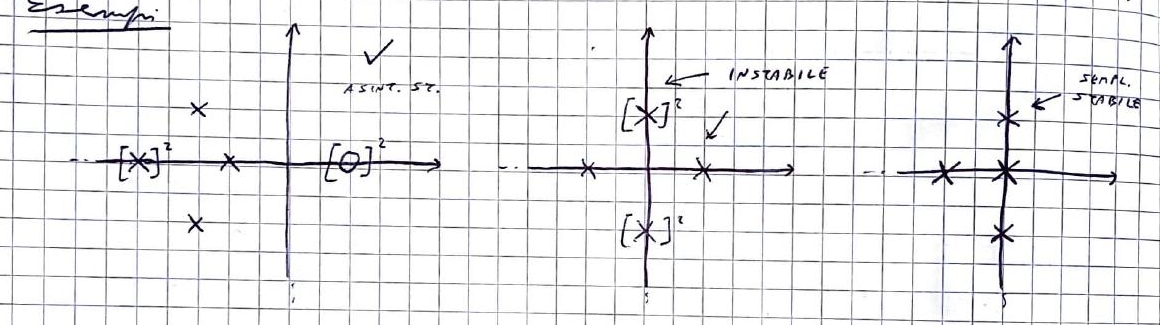
\includegraphics[width=\linewidth]{automatica_mod_1_tex_assets/b36_p36_1.png}\end{center}
\subsection*{Stabilità BIBO (Bounded Input Bounded Output)}
Per ogni $u(t)$ limitato in ampiezza esiste $y(t)$ limitata in ampiezza.
\[
\text{Un sistema è stabile BIBO}\quad\Longleftrightarrow\quad g(t)\to0.
\]
Stabilità BIBO $=$ sistema asintoticamente stabile.
\subsection*{Analisi della stabilità di un sistema ad anello chiuso}
\begin{center}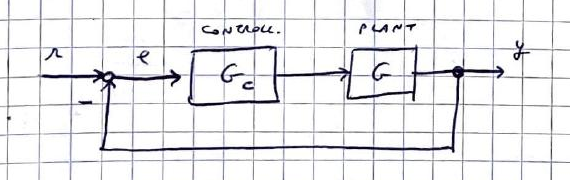
\includegraphics[width=.7\linewidth]{automatica_mod_1_tex_assets/b36_p36_2.png}\end{center}
\[
G(s)=\frac{b(s)}{a(s)}=k\frac{\prod_{i=1}^{m}(s-z_i)}{\prod_{i=1}^{n}(s-p_i)}.
\]
\begin{align*}
G_0(s)&=\frac{G_c(s)G(s)}{1+G_c(s)G(s)}\\
&=\frac{\frac{b_c(s)}{a_c(s)}\frac{b(s)}{a(s)}}
{1+\frac{b_c(s)}{a_c(s)}\frac{b(s)}{a(s)}}
=\frac{b_c(s)b(s)}{a_c(s)a(s)+b_c(s)b(s)}.
\end{align*}
$\text{Zeri di }G_0(s)$: quelli del numeratore $b_c(s)b(s)$.
% Pagina originale 37
\pagina{37}
La retroazione non sposta gli zeri, sposta i poli.
I nuovi poli sono le soluzioni dell'equazione caratteristica $a_0(s)=0$.
$a_0(s)$ è il polinomio caratteristico:
\[
a_0(s)=a(s)a_c(s)+b_c(s)b(s)=0.
\]
\subsection*{Lemma di Routh}
Condizione necessaria, non sufficiente, per la stabilità asintotica di un sistema LTI è che il polinomio caratteristico abbia tutti i coefficienti dello stesso segno e non nulli.
Negando l'affermazione precedente troviamo una condizione sufficiente affinché il sistema non sia asintoticamente stabile: basta un coefficiente nullo o discorde dagli altri.
\subsection*{Criterio di Routh--Hurwitz}
\[
a_0(s)=a_ns^n+a_{n-1}s^{n-1}+a_{n-2}s^{n-2}+a_{n-3}s^{n-3}+\cdots+a_1s+a_0.
\]
\[
\begin{array}{c|cccccc}
n&a_n&a_{n-2}&\cdots&\cdots&a_0&0\\
n-1&a_{n-1}&a_{n-3}&\cdots&\cdots&0&0\\
n-2&b_{n-2}&b_{n-4}&\cdots&\cdots&0&0\\
n-3&c_{n-3}&c_{n-5}&\cdots&\cdots&0&0\\
\vdots&\vdots&\vdots&\cdots&\cdots&\vdots&\vdots\\
1&\cdots&\cdots&0&0&0&0\\
0&\cdots&0&0&0&0&0
\end{array}
\]
\[
b_{n-2}=-\frac{\begin{vmatrix}a_n&a_{n-2}\\a_{n-1}&a_{n-3}\end{vmatrix}}{a_{n-1}},
\qquad b_{n-4}=-\frac{\begin{vmatrix}a_n&a_{n-4}\\a_{n-1}&a_{n-5}\end{vmatrix}}{a_{n-1}},
\]
\[
c_{n-3}=-\frac{\begin{vmatrix}a_{n-1}&a_{n-3}\\b_{n-2}&b_{n-4}\end{vmatrix}}{b_{n-2}},
\qquad c_{n-5}=-\frac{\begin{vmatrix}a_{n-1}&a_{n-5}\\b_{n-2}&b_{n-6}\end{vmatrix}}{b_{n-2}}.
\]
La prima colonna è chiamata sequenza di Routh:
\[
S_{\mathrm{Routh}}=(a_n,a_{n-1},b_{n-2},c_{n-3},d_{n-4},\ldots,y_{n-1},z_0).
\]
% Pagina originale 38
\pagina{38}
\subsection*{Teorema di Routh--Hurwitz}
Per ogni variazione di segno nella sequenza di Routh corrisponde una radice di $a_0(s)$ a parte reale positiva.
Per ogni permanenza di segno corrisponde una radice a parte reale negativa.
\paragraph{Esempio}
\[
S=(3,-3,4,5,-1,3).
\]
Variazioni: $3\to-3$, $-3\to4$, $5\to-1$, $-1\to3$ ($p_1,p_2,p_4,p_5>0$); permanenza: $4\to5$ ($p_3<0$).
Ci sono quattro poli positivi ed uno negativo.
Un sistema LTI è asintoticamente stabile se ogni elemento della sequenza di Routh ha sempre lo stesso segno.
Se il primo elemento di una riga è nullo posso sostituire a zero $\varepsilon>0$ e calcolare i termini della riga successiva senza dividere per $\varepsilon$ il risultato e sostituendo $\varepsilon$ con zero.
Se ho frazioni posso moltiplicare tutta la riga per un numero reale positivo.
Posso sommare una riga per se stessa traslata di $h$ posizioni e moltiplicata per $(-1)^h$.
Se ho una riga tutta nulla questa sarà per forza in posizioni dispari (se fosse in posizione pari ho $a_0=0$ e quindi posso raccogliere $s$ e fare Routh su $\widetilde a(s)=a(s)/s$).
Posso sostituire l'equazione della riga sopra con $p(s)=b(s)$, calcolarmi la derivata in $s$ e mettere i coefficienti nella riga tutta nulla.
% La notazione manoscritta accanto a b(s) nella regola della riga nulla è poco chiara; la procedura e il simbolo b(s) sono riportati fedelmente.
% Pagina originale 39
\pagina{39}
\subsection*{Stabilità di un sistema con parametri}
Affronto questa parte con esempi pratici.
\[
G(s)=\frac1{s(s+1)(s+2)}.
\]
\begin{center}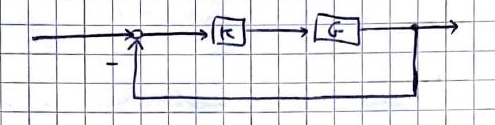
\includegraphics[width=.72\linewidth]{automatica_mod_1_tex_assets/b36_p39_1.png}\end{center}
\begin{align*}
G_0(s)&=\frac{kG}{1+kG}=\frac{k}{s(s+1)(s+2)+k}
=\frac{k}{s^3+3s^2+2s+k},\\
a_0(s)&=s^3+3s^2+2s+k.
\end{align*}
\[
\begin{array}{c|ccc}
3&1&2&0\\2&3&k&0\\1&6-k&0&0\\0&k&0&0
\end{array},\qquad
b=-\frac{\begin{vmatrix}1&2\\3&k\end{vmatrix}}3=\frac{6-k}{3},
\qquad b'=3b=6-k.
\]
\[
S=(1,3,6-k,k).
\]
È stabile se $k\in(0,6)$.
\[
\begin{array}{c|ccc}
&k<0&0<k<6&k>6\\\hline
1&+&+&+\\3&+&+&+\\6-k&+&+&-\\k&-&+&+
\end{array}
\]
$k<0$: instabile con un polo positivo; $0<k<6$: stabile; $k>6$: instabile con due poli positivi.
Trovo i valori zero e sei:
\[
k=0\quad\Longrightarrow\quad
 a_0(s)=s^3+3s^2+2s=s(s^2+3s+2)=s(s+2)(s+1).
\]
Semplicemente stabile.
\[
k=6\quad\Longrightarrow\quad a_0(s)=s^3+3s^2+2s+6.
\]
\[
\begin{array}{c|cc}3&1&2\\2&3&6\\1&3&0\\0&6&0\end{array},
\qquad b(s)=3s^2+6,
\qquad b(z)=3z+6\xrightarrow{=0}z=-2,
\qquad b'(z)=3.
\]
\[
p=\pm j\sqrt2.
\]
\begin{center}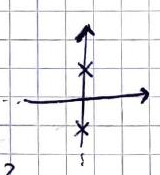
\includegraphics[width=.25\linewidth]{automatica_mod_1_tex_assets/b36_p39_2.png}\end{center}
Semplicemente stabile: tutte permanenze, ma elemento nullo in $S$, quindi non è asintoticamente stabile.
% Pagina originale 40
\pagina{40}
\subsection*{Precisione dei sistemi di controllo a regime permanente}
\begin{center}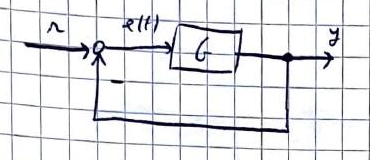
\includegraphics[width=.55\linewidth]{automatica_mod_1_tex_assets/b36_p40_1.png}\end{center}
Assumo che il sistema sia asintoticamente stabile.
Suppongo un sistema con retroazione unitaria $H(s)=1$.
Valuto l'errore a regime:
\[
e(\infty)=\lim_{s\to0}sE(s).
\]
\begin{align*}
Y(s)&=G(s)E(s)\quad\Longrightarrow\quad E(s)=\frac{Y(s)}{G(s)},\\
Y(s)&=G_0(s)R(s)=\frac{G(s)}{1+G(s)}R(s)
\quad\Longrightarrow\quad E(s)=\frac1{1+G(s)}R(s).
\end{align*}
I poli di $E(s)$ sono gli stessi di $G_0(s)$ più quelli di $R(s)$.
$E(s)$ è instabile se $G_0(s)$ è instabile.
Definisco tre errori:
\begin{itemize}
\item errore di posizione: $r(t)=1(t)$, $e_p$;
\item errore di velocità: $r(t)=t\,1(t)$, $e_v$;
\item errore di accelerazione: $r(t)=\frac{t^2}{2}\,1(t)$, $e_a$.
\end{itemize}
\subsection*{Errore di posizione $e_p$}
\[
e(\infty)=\lim_{s\to0}sE(s)
=\lim_{s\to0}s\frac1{1+G(s)}R(s)
=\frac1{1+G(s)}\mathrel{\triangleq}k_p.
\]
% La prima catena manoscritta attribuisce k_p a 1/(1+G(s)); sotto definisce k_p=G(0). Entrambe le righe sono conservate.
\[
k_p=\lim_{s\to0}G(s)=G(0)\qquad\text{costante di posizione},
\]
\[
e(\infty)=\frac1{1+k_p}\qquad\left(=\frac1{1+k_pH(s)}\right).
\]
Se $\mu=0$ ($\mu$ è il tipo del sistema: il numero di poli nell'origine di $G(s)$), $G(0)\in\mathbb R$.
Se $\mu\geq1$:
\[
G(0)=\lim_{s\to0}k\frac{\prod_i(s-z_i)}{s\prod_i(s-p_i)}=\infty.
\]
Quindi
\[
k_p\to\infty\quad\Longrightarrow\quad
 e(\infty)=\frac1{1+k_p}\to0.
\]
% Pagina originale 41
\pagina{41}
\[
e_p(\infty)=\begin{cases}\frac1{1+G(0)}&\mu=0,\\0&\mu\geq1,\end{cases}
\qquad\text{quando }r(t)=1(t).
\]
\subsection*{Errore di velocità $e_v$}
\[
E(s)=\frac1{1+G(s)}\frac1{s^2}.
\]
\begin{align*}
e(\infty)&=\lim_{s\to0}\frac1{1+G(s)}\cdot\frac1s
=\lim_{s\to0}\frac1{s+sG(s)}
=\lim_{s\to0}\frac1{sG(s)},\\
k_v&\mathrel{\triangleq}\lim_{s\to0}sG(s),\qquad
 e(\infty)=e_v=\frac1{k_v}.
\end{align*}
\begin{align*}
\mu=0&:\quad k_v=0\quad\Longrightarrow\quad e_v(\infty)\to\infty,\\
\mu=1&:\quad k_v=\lim_{s\to0}s\frac1s\overline G(s)=\overline G(0)\in\mathbb R,
\quad e(\infty)=\frac1{\overline G(0)}\in\mathbb R,\\
\mu\geq2&:\quad k_v=\lim_{s\to0}s\frac1{s^2}\overline G(s)=\infty
\quad\Longrightarrow\quad e(\infty)\to0.
\end{align*}
\[
e(\infty)=\begin{cases}\infty&\mu=0,\\\frac1{\overline G(0)}&\mu=1,\\0&\mu\geq2.\end{cases}
\]
\subsection*{Errore di accelerazione $e_a$}
\[
E(s)=\frac1{1+G(s)}\frac1{s^3}.
\]
\[
e(\infty)=\lim_{s\to0}sE(s)
=\frac1{1+G(s)}\cdot\frac1{s^2}
=\lim_{s\to0}\frac1{s^2G(s)},
\qquad k_a\mathrel{\triangleq}\lim_{s\to0}s^2G(s),\qquad e(\infty)=\frac1{k_a}.
\]
\begin{align*}
\mu=0&\Longrightarrow k_a=0\Longrightarrow e(\infty)\to\infty,\\
\mu=1&\Longrightarrow k_a=0\Longrightarrow e(\infty)\to\infty,\\
\mu=2&\Longrightarrow k_a=\overline G(0)\Longrightarrow
 e(\infty)=\frac1{\overline G(0)}\in\mathbb R,\\
\mu\geq3&\Longrightarrow k_a\to\infty\Longrightarrow e(\infty)\to0.
\end{align*}
% Pagina originale 42
\pagina{42}
\[
\begin{array}{c|cccc}\mu&0&1&2&3\\\hline
 e_p&\frac1{1+G(0)}&0&0&0\\
 e_v&\infty&\frac1{\overline G(0)}&0&0\\
 e_a&\infty&\infty&\frac1{\overline G(0)}&0
\end{array}
\]
\subsection*{Errore a regime permanente nei sistemi di controllo a retroazione non unitaria}
Tipicamente $H(s)$ è di tipo zero, quindi $H(0)$ è il guadagno statico.
\[
\widehat y(\infty)=H(0)y(\infty)\quad\Longrightarrow\quad H(0)=\gamma,
\qquad e(t)=r(t)-\gamma y(t).
\]
\[
e(t)=0\quad\Longrightarrow\quad y(t)=\frac{r(t)}\gamma.
\]
\begin{center}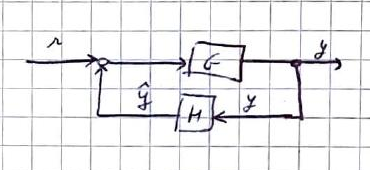
\includegraphics[width=.55\linewidth]{automatica_mod_1_tex_assets/b36_p42_1.png}\end{center}
\[
G_{\mathrm{eq}}(s)=\frac{\gamma G(s)}{1+G(s)[H(s)-\gamma]}.
\]
\paragraph{Dimostrazione}
\begin{center}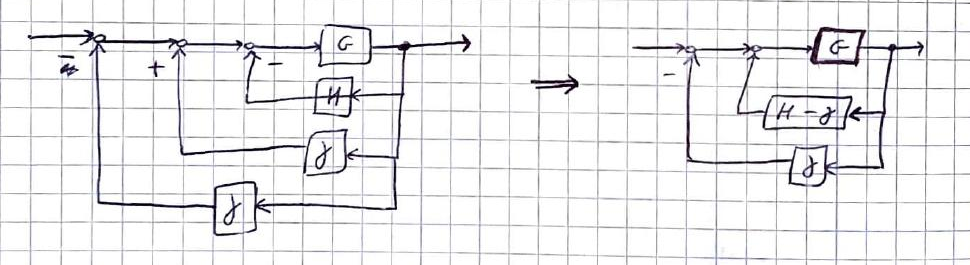
\includegraphics[width=\linewidth]{automatica_mod_1_tex_assets/b36_p42_2.png}\end{center}
\begin{center}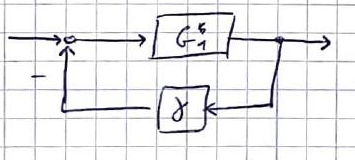
\includegraphics[width=.55\linewidth]{automatica_mod_1_tex_assets/b36_p42_3.png}\end{center}
Con
\[
G_1^\gamma=\frac G{1+G(H-\gamma)}.
\]
\begin{center}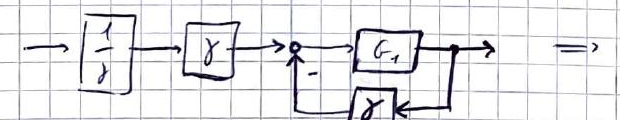
\includegraphics[width=.8\linewidth]{automatica_mod_1_tex_assets/b36_p42_4.png}\end{center}
\begin{center}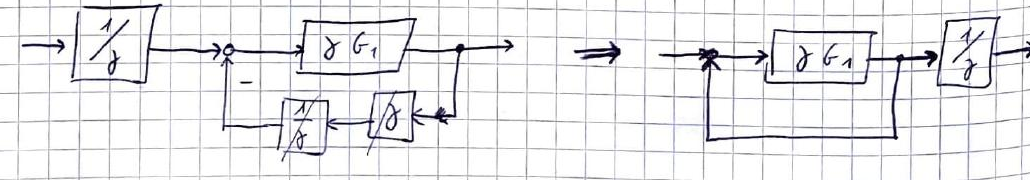
\includegraphics[width=\linewidth]{automatica_mod_1_tex_assets/b36_p42_5.png}\end{center}
% Pagina originale 43
\pagina{43}
\subsection*{Reiezione dei disturbi a regime}
Un sistema ad anello aperto non può reiettare disturbi.
\begin{center}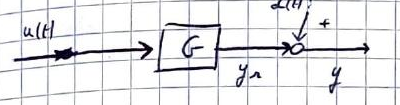
\includegraphics[width=.55\linewidth]{automatica_mod_1_tex_assets/b36_p43_1.png}\end{center}
\[
y(t)=y_r(t)+d(t),\qquad
 d(t)=1(t)\quad\Longrightarrow\quad y(\infty)=y_r(\infty)+1.
\]
Non posso reiettare nessun disturbo al di fuori dell'anello di controllo.
\begin{center}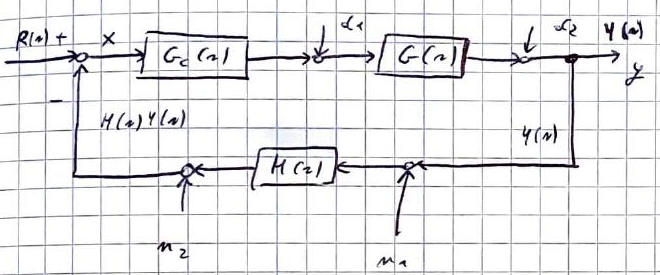
\includegraphics[width=.85\linewidth]{automatica_mod_1_tex_assets/b36_p43_2.png}\end{center}
Uso il PSE. Trovo $Y_{d_1}(s)$:
\begin{align*}
Y(s)&=[X(s)G_c(s)+D(s)]G(s),\\
Y(s)&=[(R(s)-H(s)Y(s))G_c(s)+D(s)]G(s),\\
Y(s)&=R(s)G_c(s)G(s)-H(s)Y(s)G_c(s)G(s)+D(s)G(s),\\
Y(s)(1+H(s)G_c(s)G(s))&=R(s)G_c(s)G(s)+D(s)G(s),\\
G_d(s)&=\frac{Y(s)}{D(s)}=\frac{G(s)}{1+H(s)G(s)G_c(s)}.
\end{align*}
Nel calcolo di $G_d$ pongo $R(s)=0$.
$a_0(s)$ deve avere tutti i poli nel semipiano aperto di sinistra.
Trovo
\[
Y_r(s)=\frac{G_cG}{1+HG_cG}.
\]
$Y_r(s)$ deve essere asintoticamente stabile.
Considero $D_1(s)=1/s^k$ con $k\geq1$. Vediamo per ogni $k$ quando riesco a reiettare $d_1(t)$.
% Pagina originale 44
\pagina{44}
\[
k=1,\qquad D_1(s)=\frac1s,\qquad d(t)=1(t).
\]
\[
y_{d_1}(\infty)=\lim_{s\to0}sY(s)
=\lim_{s\to0}s\frac{G(s)}{1+G(s)H(s)G_c(s)}\frac1s.
\]
Ipotizzo un polo di $G(s)$ nell'origine:
\begin{align*}
y_{d_1}(\infty)&=\lim_{s\to0}\frac{G(s)\to\infty}{1+H(s)G_c(s)G(s)}\\
&=\lim_{s\to0}\frac{G(s)}{H(s)G(s)G_c(s)}
=\lim_{s\to0}\frac1{H(s)G_c(s)}.
\end{align*}
Ipotizzo $H$ di tipo zero ($\mu_H=0$):
\[
y_{d_1}(\infty)=\frac1{H(0)}\lim_{s\to0}\frac1{G_c(s)}.
\]
Se $G_c(s)$ è di tipo zero:
\[
y_{d_1}(\infty)=\frac1{H(0)G_c(0)}\in\mathbb R.
\]
Quindi, se $G_c(s)$ è di tipo zero, $1(t)$ non è reiettabile.
Se $G_c(s)$ è di tipo uno, $y_{d_1}(\infty)=0$: se $G_c(s)$ è di tipo uno, $1(t)$ è reiettabile.
In generale: se $d_1(t)$ è di tipo $k$, è reiettabile solo se $G_c(s)$ (funzione di trasferimento a monte) è di tipo $\overline k\geq k$.
Trovo ora
\[
Y_{d_2}(s)=D_2(s)\frac1{1+HG_cG},\qquad
G_{d_2}(s)=\frac1{1+H(s)G(s)G_c(s)}.
\]
\[
y_{d_2}(\infty)=G_{d_2}(s\to0)
=\lim_{s\to0}\frac1{1+H(s)G(s)G_c(s)}.
\]
\[
y_{d_2}(\infty)\to0\quad\Longleftrightarrow\quad
G(s)G_c(s)\text{ ha almeno un polo nell'origine}.
\]
% Pagina originale 45
\pagina{45}
Generalizzando: se $d_2(t)$ è di tipo $k$, è reiettabile se è a monte di una funzione di trasferimento di tipo $\overline k\geq k$.
Solitamente il controllore ha tipo $\mu_c\geq\mu$, il tipo dell'attuatore, perché ``comanda'' quelli successivi.
\subsection*{Disturbi sul ramo di retroazione}
\begin{center}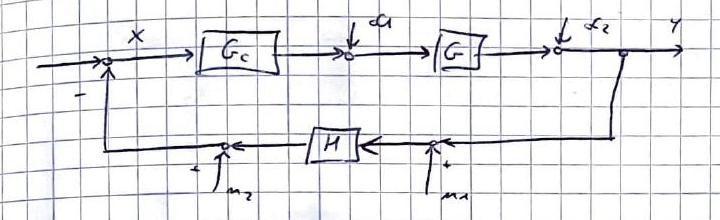
\includegraphics[width=.88\linewidth]{automatica_mod_1_tex_assets/b36_p45_1.png}\end{center}
\[
Y_{m_1}(s)=\frac{G_cGH}{1+G_cGH}.
\]
% Nella prima espressione originale manca il meno; la derivazione seguente lo include.
\begin{align*}
X(s)G_cG&=Y,\\
X(s)&=R(s)-Y(s)H(s)-N_1(s)H(s),\\
Y&=-Y(s)H(s)G_cG-N_1(s)H(s)GG_c,\\
Y(1+HG_cG)&=-N_1HG_cG,\\
Y_{m_1}&=-N_1\left(\frac{HG_cG}{1+HG_cG}\right).
\end{align*}
Se $G_c$ e $G$ devono reiettare $d_1$ e $d_2$ dovranno avere tipo $\mu\geq1$, quindi a $s\to0$:
\[
|G_cG|\gg1\qquad(G_cG\to\infty),
\]
\[
Y_{m_1}(s)\simeq-N_1
\quad\Longrightarrow\quad y_{m_1}(t)\simeq-m_1(t).
\]
Il disturbo non si può reiettare. L'unica cosa che si può fare è progettare un ramo di retroazione che abbia $m_1(t)$ piccolo.
$m_2(t)$ è fuori dal sistema ad anello chiuso:
\[
\overline r(t)=r(t)-m_2(t).
\]
Non è reiettabile.
% Pagina originale 46
\pagina{46}
\subsection*{Tecnica di precompensazione dei disturbi}
\begin{center}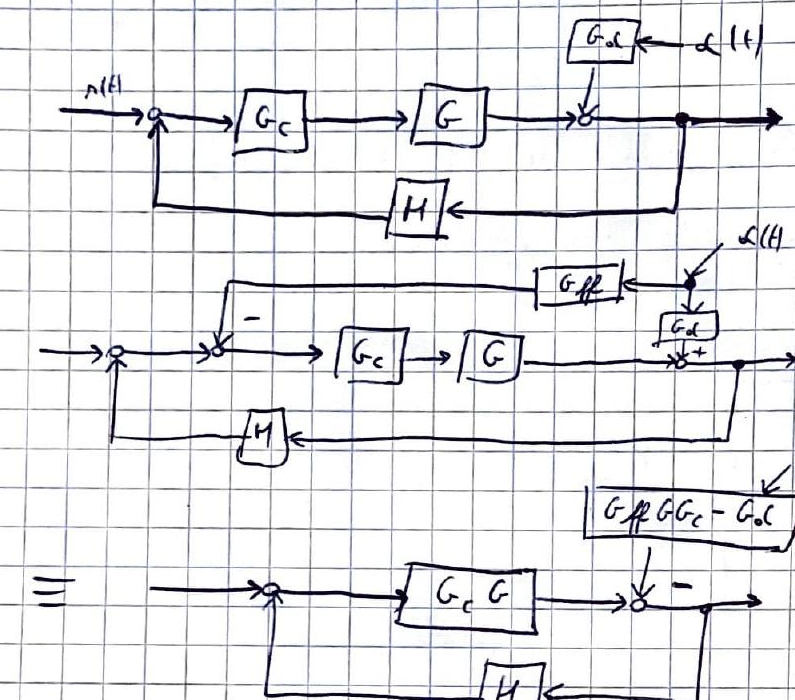
\includegraphics[width=.83\linewidth]{automatica_mod_1_tex_assets/b36_p46_1.png}\end{center}
\[
G_d=1\quad\Longrightarrow\quad d(t)=d_2(t),\qquad
G_d=G\quad\Longrightarrow\quad d(t)=d_1(t).
\]
Progetto controllori che provano ad annullare $d(t)$ prima che intervenga sul ramo diretto.
Per annullare il disturbo:
\[
G_{\mathrm{ff}}GG_c-G_d=0
\quad\Longrightarrow\quad G_{\mathrm{ff}}=\frac{G_d}{GG_c}.
\]
Ma probabilmente $GG_c$ ha il denominatore di grado maggiore di quello di $G_d$, quindi $G_{\mathrm{ff}}$ sarebbe impropria (e quindi irrealizzabile).
\paragraph{Esempio}
\[
G_d=\frac1{s+p},\qquad G_cG(s)=\frac{\omega_n^2}{s^2+2\delta\omega_ns+\omega_n^2},
\]
\[
G_{\mathrm{ff}}=\frac{s^2+2\delta\omega_ns+\omega_n^2}{(s+p)\omega_n^2},
\qquad m=2,\quad n=1,\quad m>n:\ \text{impropria}.
\]
% Pagina originale 47
\pagina{47}
\subsection*{Sensibilità alle variazioni parametriche}
\begin{center}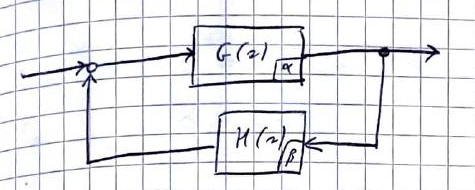
\includegraphics[width=.67\linewidth]{automatica_mod_1_tex_assets/b36_p47_1.png}\end{center}
\[
G(s;\alpha),\qquad H(s;\beta).
\]
Suppongo che il parametro abbia una certa precisione:
\[
\alpha=\underbrace{\alpha_0}_{\text{valore nominale}}
+\underbrace{\Delta\alpha}_{\text{variazione parametrica}}.
\]
Si dice sensibilità di $G(s)$ rispetto ad $\alpha$ la funzione
\[
S_\alpha^G\mathrel{\triangleq}\lim_{\Delta\alpha\to0}
\frac{\Delta G/G}{\Delta\alpha/\alpha}
=\frac{\partial G}{\partial\alpha}\frac\alpha G.
\]
\paragraph{Esempio}
\[
G(s;\alpha)=\frac1{s+\alpha}.
\]
\begin{align*}
S_\alpha^G&=\frac{\partial G}{\partial\alpha}\frac\alpha G
=-\frac1{(s+\alpha)^2}\frac\alpha G\\
&=-\frac1{(s+\alpha)^2}\frac{\alpha(s+\alpha)}1
=-\frac\alpha{s+\alpha}.
\end{align*}
\subsection*{Regola della catena}
\[
S_\alpha^\beta=S_\alpha^\delta S_\delta^\beta.
\]
\[
G(s;\alpha)\simeq G(s;\alpha_0)+\Delta G(s)
=G(s;\alpha_0)+\left.\frac{\partial G}{\partial\alpha}\right|_{\alpha=\alpha_0}\Delta\alpha.
\]
\subsection*{Luogo delle radici}
\begin{center}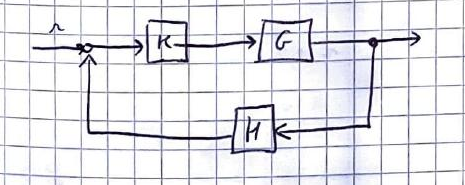
\includegraphics[width=.65\linewidth]{automatica_mod_1_tex_assets/b36_p47_2.png}\end{center}
\[
G_0(s)=\frac{kG(s)}{1+kG(s)H(s)}.
\]
Studiamo l'equazione caratteristica, $a_0=1+kGH=0$.
Si chiama luogo delle radici il luogo dei punti del piano complesso che risolvono l'equazione caratteristica
\[
1+kGH=1+kL(s)=0
\]
per tutti i valori positivi di $k$ ($k\in\mathbb R^+$).
% Pagina originale 48
\pagina{48}
Il luogo dei punti che risolvono l'equazione caratteristica con $k\in\mathbb R^-$ è chiamato luogo delle radici complementare.
\[
\overline s\in\mathrm{LdR}_+\quad\Longrightarrow\quad
\exists\overline k\in\mathbb R^+:a_0(\overline s)=0,
\]
\[
\overline s\in\mathrm{LdR}_-\quad\Longrightarrow\quad
\exists\overline k\in\mathbb R^-:a_0(\overline s)=0.
\]
Considero
\[
a_0(s)=1+kL(s)=0\quad\Longrightarrow\quad L(s)=-\frac1k
\quad\Longleftrightarrow\quad
\begin{cases}|L(s)|=|1/k|&\text{equazione di taratura},\\
\arg L(s)=\arg(-1/k)&\text{regola delle fasi}.\end{cases}
\]
\[
\arg L(s)=\arg\left(-\frac1k\right).
\]
\subsection*{Regola delle fasi}
\[
\arg L(s)=\arg\left(-\frac1k\right)
\quad\Longrightarrow\quad
\arg L(s)=\begin{cases}(2\nu+1)\pi&k>0,\\2\nu\pi&k<0.\end{cases}
\]
\begin{align*}
\arg L(s)&=\arg\frac{\prod_i(s-z_i)}{\prod_i(s-p_i)}
=\sum_i\arg(s-z_i)-\sum_i\arg(s-p_i)\\
&=\sum_{i=1}^{m}\varphi_i-\sum_{i=1}^{n}\theta_i
=\begin{cases}(2\nu+1)\pi&k>0,\ \mathrm{LdR}_+,\\
2\nu\pi&k<0,\ \mathrm{LdR}_-.\end{cases}
\end{align*}
Con $\varphi_i=\arg(s-z_i)$ e $\theta_i=\arg(s-p_i)$.
\paragraph{Esempio}
\[
L(s)=\frac{s+1}{s(s+2)},\qquad
\arg L(s)=\arg(s+1)-\arg s-\arg(s+2)
=\begin{cases}(2\nu+1)\pi&k>0,\\2\nu\pi&k<0.\end{cases}
\]
\[
\overline s=-1+j,\qquad
\overline s+1=\overline s-z_1,\quad
\overline s=\overline s-p_1,\quad
\overline s+2=\overline s-p_2,
\]
\[
z_1=-1,\qquad p_1=0,\qquad p_2=-2.
\]
\[
\arg L(\overline s)=\arg j-\arg(-1+j)-\arg(1+j)
=\frac\pi2-\frac{3\pi}4-\frac\pi4=-\frac\pi2.
\]
% Nota conclusiva manoscritta alla fine della pagina 48 non chiaramente leggibile; il calcolo è interamente trascritto.
% Pagina originale 49
\pagina{49}
\[
-\frac\pi4\ne(2\nu+1)\pi\quad\land\quad-\frac\pi4\ne2\nu\pi
\quad\Longrightarrow\quad
\overline s\notin\mathrm{LdR}_+\quad\land\quad\overline s\notin\mathrm{LdR}_-.
\]
% La pagina precedente calcola -pi/2; qui il manoscritto scrive -pi/4. Entrambi conservati.
La regola delle fasi rappresenta una verifica, non un modo per trovare le radici.
\subsection*{Equazione di taratura}
\[
|k|=\frac1{|L(s)|}=\frac{\prod_i\rho_i}{\prod_i\chi_i},
\qquad\rho_i=|s-p_i|,\quad\chi_i=|s-z_i|.
\]
$k$ aumenta allontanandosi dai poli e avvicinandosi agli zeri.
\subsection*{Regole di Evans}
\begin{enumerate}
\item Il luogo delle radici è sempre simmetrico rispetto all'asse reale.
\item Il luogo delle radici ha numero di rami pari al numero dei poli di $L(s)$.
\item Ogni polo dà origine ad un ramo ($k\to0$) che o confluisce in uno zero o diverge. Ci sono $n-m$ asintoti ad un ramo all'infinito ($n$ è il numero dei poli, $m$ il numero degli zeri).
\end{enumerate}
\begin{center}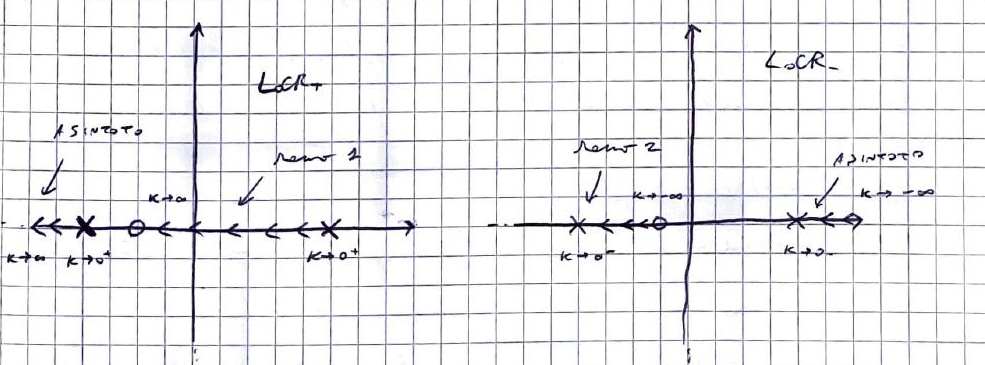
\includegraphics[width=\linewidth]{automatica_mod_1_tex_assets/b36_p49_1.png}\end{center}
\[
\lim_{s\to p}|L(s)|=\infty\quad\Longrightarrow\quad|k|\to0,
\qquad
\lim_{s\to z}|L(s)|=0\quad\Longrightarrow\quad|k|\to\infty.
\]
% Pagina originale 50
\pagina{50}
\begin{enumerate}\setcounter{enumi}{3}
\item Un punto $s\in\mathbb R$ appartiene a $\mathrm{LdR}_+$ [$\mathrm{LdR}_-$] se alla sua destra ci sono un numero dispari [pari] di poli o zeri.
\end{enumerate}
La dimostrazione viene dalla regola delle fasi.
In $\mathrm{LdR}_+$:
\[
\arg L(\overline s)=(2\nu+1)\pi.
\]
Le fasi per le coppie complesse di poli si annullano. Per ogni polo sottraggo $\pi$, per ogni zero aggiungo $\pi$:
\[
m\pi-n\pi=(m-n)\pi,
\qquad m-n\text{ dispari}=2\nu+1.
\]
Per $\mathrm{LdR}_-$, $\arg L(s)=2\nu\pi$, quindi il numero di poli e di zeri devono essere pari.
\begin{enumerate}\setcounter{enumi}{4}
\item I rami che tendono all'infinito si ritrovano tutti in un punto dell'asse reale $\sigma$, detto centroide:
\[
\sigma=\frac{\sum_i^np_i-\sum_i^mz_i}{n-m}.
\]
Gli angoli degli asintoti si calcolano come
\[
\theta_{a,\nu}=\begin{cases}
\frac{(2\nu+1)\pi}{n-m}&k>0,\ \mathrm{LdR}_+,\\
\frac{2\nu\pi}{n-m}&k<0,\ \mathrm{LdR}_-,
\end{cases}\qquad \nu\in\mathbb N.
\]
\item Ci sono punti di confluenza e punti di emersione che sono le radici multiple di $a_0(s)=1+kL(s)=0$.
Si trovano risolvendo
\[
a'(s)b(s)-a(s)b'(s)=0,\qquad L(s)=\frac{b(s)}{a(s)}.
\]
I punti di confluenza sono i punti dell'asse reale nei quali confluiscono due o più rami.
I punti di emersione sono i punti dell'asse reale dai quali emergono due o più rami.
\end{enumerate}
% Pagina originale 51
\pagina{51}
\begin{enumerate}\setcounter{enumi}{6}
\item Angolo di partenza di un ramo da un polo:
\[
\theta_{p,\nu}=\frac1r\left[
\sum_i\arg(p-z_i)-\sum_{p_i\ne p}\arg(p-p_i)
+\begin{cases}(2\nu+1)\pi&k>0,\\2\nu\pi&k<0\end{cases}\right].
\]
$r$: molteplicità.
\begin{center}
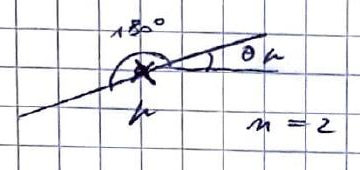
\includegraphics[width=.45\linewidth]{automatica_mod_1_tex_assets/b36_p51_1.png}\quad
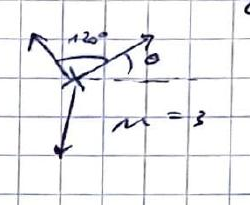
\includegraphics[width=.32\linewidth]{automatica_mod_1_tex_assets/b36_p51_2.png}
\end{center}
Molteplicità $r=2$: angoli separati di $180^\circ$; $r=3$: angoli separati di $120^\circ$.
\item Angolo di arrivo agli zeri:
\[
\theta_{z,\nu}=\frac1r\left[
\sum_i\arg(z-p_i)-\sum_{z_i\ne z}\arg(z-z_i)
+\begin{cases}(2\nu+1)\pi&k>0,\\2\nu\pi&k<0\end{cases}\right].
\]
\item Il luogo delle radici interseca l'asse immaginario per valori di $k$ che annullano una riga dispari della tabella di Routh.
\end{enumerate}
